% !TeX spellcheck = en_US
\documentclass[a4paper,11pt]{article}
\newcommand{\tg}{\mathop{\mathrm{tg}}\nolimits}
\newcommand{\divn}{\mathop{\mathrm{div}}\nolimits}
\usepackage[process=auto]{pstool}
\usepackage[english]{babel}
\usepackage[T2A]{fontenc}
\usepackage[cp1251]{inputenc}
\usepackage{amssymb,amsmath}
\usepackage{gensymb,textcomp,latexsym}
\usepackage{graphicx}
\usepackage[usenames,dvipsnames]{xcolor}
\usepackage[font=small,labelfont=bf]{caption}
\usepackage[center]{subfigure}
\usepackage[pdfauthor={Shchelik},
pdftitle={Nonorthogonal Alford test},
pdfstartview=XYZ,
bookmarks=true,
colorlinks=true,
linkcolor=blue,
urlcolor=blue,
citecolor=blue,
%pdftex,
bookmarks=true,
linktocpage=true,   % makes the page number as hyperlink in table of content
hyperindex=true]{hyperref}
%\usepackage[hyperpageref]{backref}
\usepackage[section]{placeins}
\usepackage{graphicx}
\usepackage{epsfig}
\usepackage{epstopdf}
\usepackage{subfigure}
\usepackage{float}
\usepackage{booktabs}
\graphicspath{ {./image_test/} }
\usepackage[pdftex, left=1in, right=1in, top=1in, bottom=2cm]{geometry}

\usepackage{parcolumns}
\usepackage{tikz}

\begin{document}
\section{Introduction}

\section{Methods}
A cross-dipole acoustic logging tool consists of two sets of transmitter-receiver arrays, each pointing to one of orthogonal directions associated with the tool. During measurement procedure these arrays form four-component dipole data which include two in-line components and two cross-line components, that corresponds to various mutual orientation of active source and receivers. In classics each of these components is a linear combination of two orthogonally polarized wave modes which propagates along borehole without interaction. Due to principle of reciprocity the cross-line components should be equal and therefore the $2\times 2$ matrix $\mathbf{R}$ consisting of measurement data components could be represented in the following form

\begin{equation}
\mathbf{R} = \mathbf{P} \ \mathbf{D} \ \mathbf{P}^T, \label{eq:alford_symmetric} 
\end{equation}
where $\mathbf{D}$ -- diagonal matrix which corresponds to the pure modes propagation. In the canonical symmetric Alford rotation \cite{Alford1986} procedure the transformation matrix $\mathbf{P}$ is just a rotation matrix on angle $\theta$

\begin{equation*}
\mathbf{P} = \left\|
\begin{array}{cc}
\cos \theta &-\sin \theta \\ 
\sin \theta & \cos \theta
\end{array} 
\right\| 
\end{equation*}

The real data matrix $\mathbf{R}$ is usually not symmetrical, therefore rotation angle $\theta$ is found by minimization of non-diagonal components of $\mathbf{D}$. Though the considered algorithm is very effective and stable in many practical cases it also contain some fundamental drawbacks. For instance, the particle-motion directions associated with shear waves propagating in arbitrary ray directions in orthorhombic media need not be orthogonal, so the data matrix can't be diagonalized with Alford rotation transformations. However, \cite{Dellinger1997} showed that data matrix recorded by a cross-dipole logging tool should be symmetric regardless of heterogeneity and anisotropy. They proposed a symmetric generalization of Alford rotation procedure which involve minimization by two angles $\theta$ and $\eta$ for corresponding transformation matrix 
\begin{equation*}
\mathbf{P} = \left\|
\begin{array}{cc}
\cos \theta & -\sin (\theta+\eta) \\ 
\sin \theta & \cos (\theta+\eta)
\end{array} 
\right\|
\end{equation*}

For the given recorder data matrix $\mathbf{R}$ the values for $\theta$ and $\eta$ are chosen to minimize the sum of the squares of the off-diagonal entries of $\mathbf{D}$, averaged over the full waveform (no time window). If $\eta=0$ method reduces to standard Alford rotation.

\section{Models description}

\begin{minipage}[c]{0.47\linewidth}	
\begin{center}
		Borehole geometry \\
		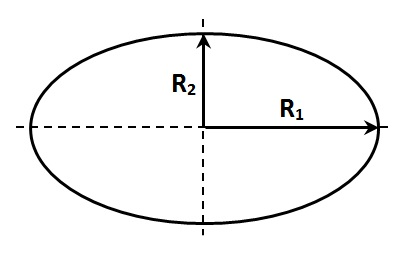
\includegraphics[width=1\linewidth]{./images/nonorth_alford/scheme_bh_image_hr.jpg}	  
\end{center}	  		
\end{minipage} \hfill
\begin{minipage}[c]{0.47\linewidth}
\begin{center}
		TI axis orientation\\
			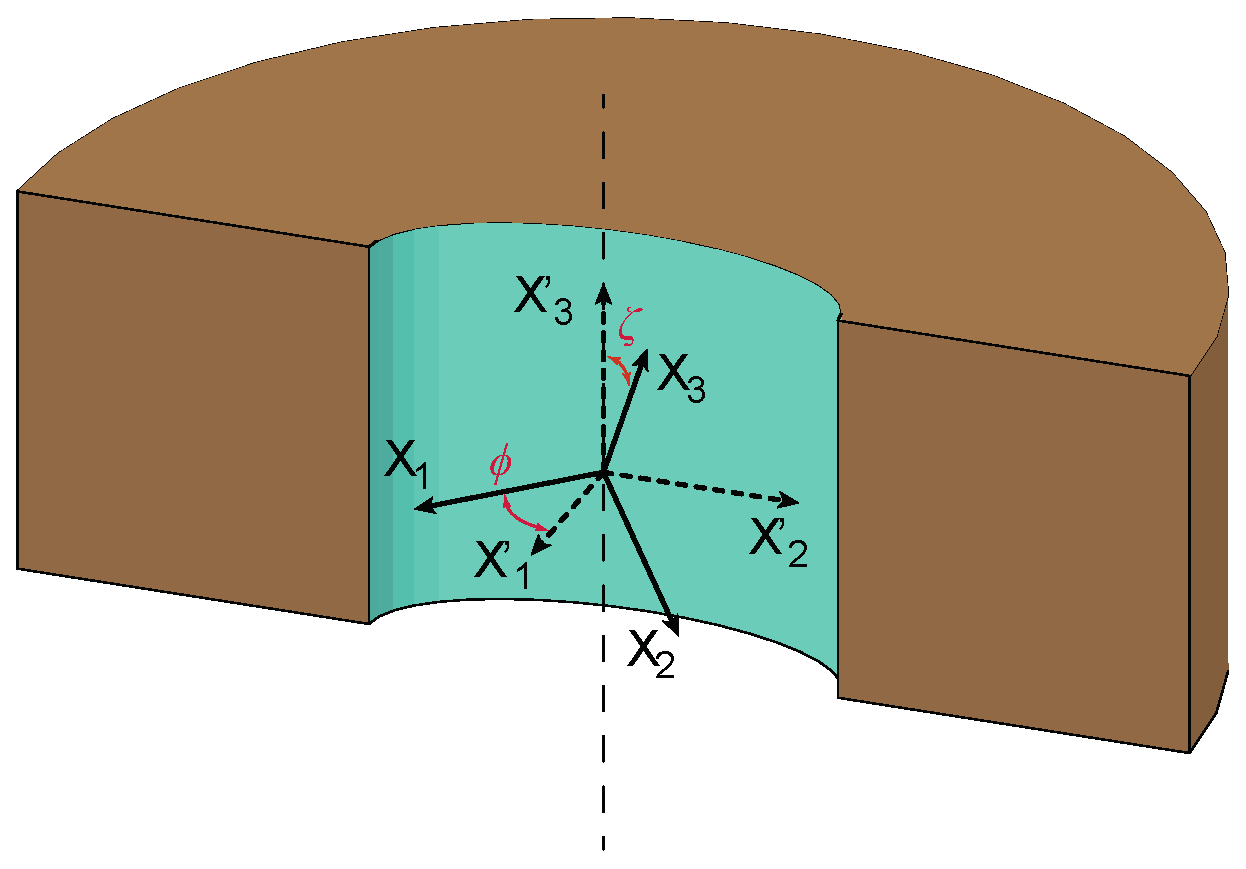
\includegraphics[width=1\linewidth]{./images/nonorth_alford/TI_axes_desc.eps}		
\end{center}
\end{minipage}

\begin{description}
\item[Model 1:] Cylindrical borehole  $R_1=R_2=20$ cm, Austin Chalk (TI angles: $\zeta=60$\textdegree, $\phi=45$\textdegree)
\item[Model 2:] Elliptical borehole $R_1=15$ cm, $R_2=10$ cm, Isotropic slow formation ($\rho=2000$ kg/m$^3$, $V_p=2545$ m/s, $V_s=1018$ m/s) 
\item[Model 3:] Elliptical borehole $R_1=20$ cm, $R_2=10$ cm, Austin Chalk (TI angles: $\zeta=60$\textdegree, $\phi=45$\textdegree) 
\end{description}

\section{Results}
\subsection*{Raw data processing}

\renewcommand{\arraystretch}{1.5}
\footnotesize
\begin{tabular}{c|rr|rr|r|ll}
				&\multicolumn{1}{c}{$\theta_1^o$} & \multicolumn{1}{c|}{$\theta_1^n$} & \multicolumn{1}{c}{$\theta_2^o$} & \multicolumn{1}{c|}{$\theta_2^n$} & \multicolumn{1}{c|}{$\Delta\theta^n$}& \multicolumn{1}{c}{$E_{cross}^o/E_{total}^o$} & \multicolumn{1}{c}{$E_{cross}^n/E_{total}^n$} \\ \hline
\hline Model 1 & -44.9996 & -44.9998 & 45.0004 & 45.0003 & ~0 & $3.1640 \cdot 10^{-10}$ & $3.1385 \cdot 10^{-10}$ \\ 
	   Model 2 & -0.0125 & -0.0127 & -90.0125 & -90.0082 & ~0 & $5.1932 \cdot 10^{-6}$ & $5.1901 \cdot 10^{-6}$ \\ 
 	   Model 3 & \textbf{-10.5111} & \textbf{-26.3606} & \textbf{79.4889} & \textbf{80.4622} & \textbf{16.8228} & \color{red}{\textbf{0.1726}} & \color{red}{\textbf{0.1511}} \\
 	    \hline 
\end{tabular} 
\\ \\
\quad *$E_{total}$ denotes 1-norm of the corresponding $\mathbf{D}$ matrix.
\renewcommand{\arraystretch}{1.0}
\normalsize
\vspace{\baselineskip}

\textbf{Plot of TI axis direction obtained for Model 3}\\

\begin{minipage}[c]{0.47\linewidth}	
\begin{center}
		Orthogonal Alford rotation \\
		\psfragfig[width=0.40\linewidth,crop=pdfcrop]{./images/nonorth_alford/el20x10_TTI60_rot4c_scheme}	  		
\end{center}	  		
\end{minipage} 
\begin{minipage}[c]{0.47\linewidth}
\begin{center}
		Non-orthogonal Alford rotation\\
			\psfragfig[width=0.40\linewidth,crop=pdfcrop]{./images/nonorth_alford/el20x10_TTI60_gs_rot4c_scheme}			
\end{center}
\end{minipage} \\
\footnotesize Here blue lines denote directions obtained from Alford processing; black arrows --- initial direction of dipole sources in numerical calculations.
\normalsize
\vspace{\baselineskip}
\vspace{\baselineskip} 

\begin{minipage}[h]{0.47\linewidth}	
\begin{center} 
$E_{cross}$ function dependence on $\theta$ and $\eta$ (Model 3)\\
			\psfragfig[width=0.40\linewidth,crop=pdfcrop]{./images/nonorth_alford/solution_min_gs_rot4c}
			\label{fig:rot4_gs_solution}
\end{center}
\end{minipage} \hfill
\begin{minipage}[h]{0.47\linewidth}
\begin{center}
TKO processing of the rotated waveforms (Model 3)
			\psfragfig[width=0.40\linewidth,crop=pdfcrop]{./images/nonorth_alford/el20x10_TTI60_TKO_compare}\\
	  		\label{fig:rot4_tko_comp}
\end{center}	  		
\end{minipage}

\newpage

\subsection*{Processing with filters and time window}

Two filters or time window were applied to raw Model 3 data before processing.

\begin{description}
\item[Filter parameters:] Sampling frequency 1194892 Hz, $A_{pass} = 1$ dB, $A_{stop} = 80$ dB, \\ Low-pass: $F_{stop} = 4000$ Hz, $F_{pass} = 5000$ Hz \\ High-pass: $F_{pass} = 4000$ Hz, $F_{stop} = 5000$ Hz
\item[Window parameters:] width $\Delta t=1$ ms, slowness $s = 987$ mcs/m
\end{description}

\renewcommand{\arraystretch}{1.5}
\footnotesize
\begin{tabular}{c|rr|rr|r|ll}
				&\multicolumn{1}{c}{$\theta_1^o$} & \multicolumn{1}{c|}{$\theta_1^n$} & \multicolumn{1}{c}{$\theta_2^o$} & \multicolumn{1}{c|}{$\theta_2^n$} & \multicolumn{1}{c|}{$\Delta\theta^n$}& \multicolumn{1}{c}{$E_{cross}^o/E_{total}^o$} & \multicolumn{1}{c}{$E_{cross}^n/E_{total}^n$} \\ \hline
\hline  Model 3 (raw) & -10.5111 & -26.3606 & 79.4889 & 80.4622 & 16.8228 & 0.1726 & 0.1511 \\
		Time window & -31.0135 & -42.6876 & 58.9865 & 67.8336 & 20.5212& \color{red}{0.0445} & \color{red}{0.0099} \\
	   Low-pass filter & -30.6596 & -41.5868 & 59.3404 & 68.1357 & 19.7225 & \color{red}{0.0358} & \color{red}{0.0027} \\
 	   High-pass filter & -1.7554 & -4.9971 & 88.2446 & 88.5870 & 3.5841& \color{red}{0.0602} & \color{red}{0.0597} \\ 	   
 	    \hline 
\end{tabular} 
\normalsize
\\ \\
\quad *$E_{total}$ denotes 1-norm of the corresponding $\mathbf{D}$ matrix.
\renewcommand{\arraystretch}{1.0}

\vspace{\baselineskip}

\textbf{Plot of TI axis direction}\\

\begin{minipage}[c]{0.47\linewidth}
\begin{center}
		Time window plot\\
			\psfragfig[width=0.47\linewidth,crop=pdfcrop]{./images/nonorth_alford/el20x10_TTI60_traces_twindow_1ms}
		
\end{center}
\end{minipage}	
\begin{minipage}[c]{0.47\linewidth}
\begin{center}
		Non-orthogonal Alford rotation with time window 1 ms\\
			\psfragfig[width=0.40\linewidth,crop=pdfcrop]{./images/nonorth_alford/el20x10_TTI60_gs_rot4c_twindow_1ms}
		
\end{center}
\end{minipage} \hfill	 \\
\begin{minipage}[c]{0.47\linewidth}	
\begin{center}
		Non-orthogonal Alford rotation with lowpass filter\\
		\psfragfig[width=0.40\linewidth,crop=pdfcrop]{./images/nonorth_alford/el20x10_TTI60_gs_rot4c_lpfilter}			
	  		\label{fig:rot4_gs_lp_scheme}
\end{center}	  		
\end{minipage}
\begin{minipage}[c]{0.47\linewidth}
\begin{center}
		Non-orthogonal Alford rotation with highpass filter\\
			\psfragfig[width=0.40\linewidth,crop=pdfcrop]{./images/nonorth_alford/el20x10_TTI60_gs_rot4c_hpfilter}
			\label{fig:rot4_gs_hp_scheme}
\end{center}
\end{minipage} \\

\footnotesize Here blue lines denote directions obtained from Alford processing; black arrows --- initial direction of dipole sources in numerical calculations.
\normalsize

\vspace{\baselineskip}
\vspace{\baselineskip}

\subsection*{Processing results for other cases}

\begin{description}
\item[Model 4:] Elliptical $R_1=15$ cm, $R_2=10$ cm, Austin Chalk (TI angles: $\zeta=60$\textdegree, $\phi=45$\textdegree) 
\item[Model 5:] Elliptical $R_1=15$ cm, $R_2=10$ cm, Cotton Valey Shale (TI angles: $\zeta=60$\textdegree, $\phi=45$\textdegree) 
\item[Model 6:] Elliptical $R_1=20$ cm, $R_2=10$ cm, Cotton Valey Shale (TI angles: $\zeta=60$\textdegree, $\phi=45$\textdegree) 
\end{description}

\begin{description}
\item[Filter parameters:] Sampling frequency 1194892 Hz, $A_{pass} = 1$ dB, $A_{stop} = 80$ dB, \\ Low-pass: $F_{stop} = 4000$ Hz, $F_{pass} = 5000$ Hz \\ High-pass: $F_{pass} = 4000$ Hz, $F_{stop} = 5000$ Hz
\item[Window 1 parameters:] width $\Delta t=1$ ms, slowness $s = 987$ mcs/m
\item[Window 2 parameters:] width $\Delta t=0.5$ ms, slowness $s = 400$ mcs/m
\end{description}

\renewcommand{\arraystretch}{1.5}
\footnotesize
\begin{tabular}{c|rr|rr|r|ll}
				&\multicolumn{1}{c}{$\theta_1^o$} & \multicolumn{1}{c|}{$\theta_1^n$} & \multicolumn{1}{c}{$\theta_2^o$} & \multicolumn{1}{c|}{$\theta_2^n$} & \multicolumn{1}{c|}{$\Delta\theta^n$}& \multicolumn{1}{c}{$E_{cross}^o/E_{total}^o$} & \multicolumn{1}{c}{$E_{cross}^n/E_{total}^n$} \\ \hline
\hline  Model 4 (raw) & -33.1254 & -43.2920 & 56.8746 & 65.1455 & 18.4 & 0.0791 & 0.0460 \\
		Time window 1 & -34.9269 & -42.3895 & 55.0731 & 62.0447 & 14.4 & 0.0113 & 0.0010 \\
	   Low-pass filter & -34.8496 & -42.1434 & 55.1538 & 62.0865 & 14.2 & 0.0117 & 0.0005 \\
 	   High-pass filter & -13.8552 & -30.2318 & 76.1448 & 75.9994 & 16.2 & 0.1489 & 0.1250 \\ 	   
 	    \hline 
\end{tabular} 
\normalsize
\renewcommand{\arraystretch}{1.0}

\vspace{\baselineskip}

\renewcommand{\arraystretch}{1.5}
\footnotesize
\begin{tabular}{c|rr|rr|r|ll}
				&\multicolumn{1}{c}{$\theta_1^o$} & \multicolumn{1}{c|}{$\theta_1^n$} & \multicolumn{1}{c}{$\theta_2^o$} & \multicolumn{1}{c|}{$\theta_2^n$} & \multicolumn{1}{c|}{$\Delta\theta^n$}& \multicolumn{1}{c}{$E_{cross}^o/E_{total}^o$} & \multicolumn{1}{c}{$E_{cross}^n/E_{total}^n$} \\ \hline
\hline  Model 5 (raw) & -88.2731 & -88.2149 & 1.7269 & 1.6286 & 0.15 & 0.0041 & 0.0041 \\
		Time window 2 & -53.6211 & -62.9063 & 36.3789 & 49.2159 & 22.1 & 0.1951 & 0.1362 \\
	   Low-pass filter & -87.7936 & -73.4542 & 2.2064 & 2.1189 & 14.4 & 0.0107 & 0.0084 \\ 	   
 	    \hline 
\end{tabular} 
\normalsize
\renewcommand{\arraystretch}{1.0}

\vspace{\baselineskip}

\renewcommand{\arraystretch}{1.5}
\footnotesize
\begin{tabular}{c|rr|rr|r|ll}
				&\multicolumn{1}{c}{$\theta_1^o$} & \multicolumn{1}{c|}{$\theta_1^n$} & \multicolumn{1}{c}{$\theta_2^o$} & \multicolumn{1}{c|}{$\theta_2^n$} & \multicolumn{1}{c|}{$\Delta\theta^n$}& \multicolumn{1}{c}{$E_{cross}^o/E_{total}^o$} & \multicolumn{1}{c}{$E_{cross}^n/E_{total}^n$} \\ \hline
\hline  Model 6 (raw) & -89.1579 & -89.1352 & 0.8421 & 0.7691 & 0.1 & 0.0062 & 0.0062 \\
		Time window 2 & -29.3221 & -59.0992 & 60.6779 & 62.8873 & 32.0 & 0.3304 & 0.2324 \\
	   Low-pass filter & -89.0481 & -75.6149 & 0.9519 & 0.9021 & 13.5 & 0.0025 & 0.0021 \\ 	   
 	    \hline 
\end{tabular} 
\normalsize
\\ \\
\quad *$E_{total}$ denotes 1-norm of the corresponding $\mathbf{D}$ matrix.
\renewcommand{\arraystretch}{1.0}

\vspace{\baselineskip}

\newpage

\subsection*{Filter description}

\begin{minipage}[h]{0.47\linewidth}	
\begin{center} 
\textbf{Lowpass filter scheme}\\
			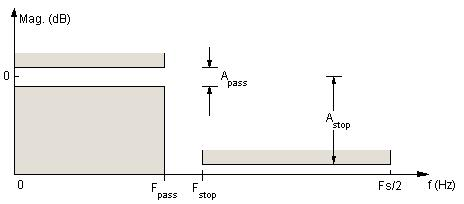
\includegraphics[width=\linewidth]{./images/nonorth_alford/lowpass_filter_scheme}
			
\end{center}
\end{minipage} \hfill
\begin{minipage}[h]{0.47\linewidth}
\begin{center}
\textbf{Lowpass filter magnitude response}
			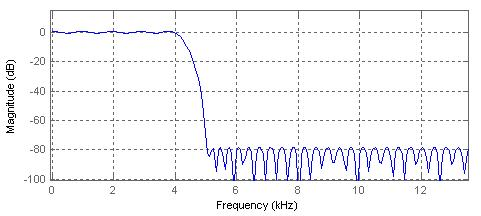
\includegraphics[width=\linewidth]{./images/nonorth_alford/lowpass_margn_response}\\
	  		
\end{center}	  		
\end{minipage}

\begin{minipage}[h]{0.47\linewidth}	
\begin{center} 
\textbf{Highpass filter scheme}\\
			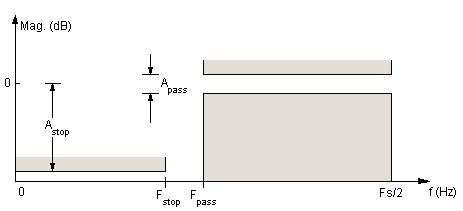
\includegraphics[width=\linewidth]{./images/nonorth_alford/highpass_filter_scheme}
			
\end{center}
\end{minipage} \hfill
\begin{minipage}[h]{0.47\linewidth}
\begin{center}
\textbf{Highpass filter magnitude response}
			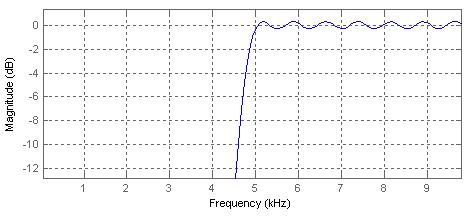
\includegraphics[width=\linewidth]{./images/nonorth_alford/highpass_margn_response}\\
	  		
\end{center}	  		
\end{minipage}

\vspace{\baselineskip}
\vspace{\baselineskip} 

\include{nonorth_alford_SAFE}

%\bibliography{./library/library}
\bibliography{../../../Literature/TeX_Library/library}
\bibliographystyle{unsrt}
%\bibliographystyle{plainnat_no_url}



\end{document} 